% This section shows the development and justification of the design of your artefact from requirements through to final design.
% \section{Research}
% \subsection{In-band management systems}
% \subsection{Out-of-band management systems}
\section{Methodology}
\label{section:design-methodology}
As chapter \ref{chap:litreview} proves, little academic research exists around out-of-band management of network devices, and specifically the security risks associated with it. Therefore, an inductive approach was taken during the research phase to create a base theory that was used as part of the evaluation of the finished product. \\\\
The Kanban development and task management methodology was used during this project. Kanban was designed originally for software development, where a list of tasks is kept in a Backlog, and developers pull tasks from this list into their 'in progress' queue. Once a task is complete, the developer will move the task into either a 'in review' queue, or a 'complete' queue. This allows the entire development team to easily visualise the status of tasks in the project. \\\\
While Kanban is designed for software development, in the case of this project, no software was developed so this system was used to easily see what tasks were completed and what still needed to be done. It was mainly used during the design and development phases. When designing the final product, functionality and security ideas were added to an 'Ideas' column, similar to the 'Backlog' in standard Kanban. If an idea was selected it was moved to a 'Confirmed' column, while other ideas were moved to a 'Rejected' column. This helped to prevent repetition of ideas during the design phase, and allowed previously rejected ideas to be approved if it was found that they were actually needed.

\subsection{Possible approaches}
\label{subsection:design-methodology-approaches}
Three potential approaches to the problem were identified and are described below. The project proposal issued by Multi-Tech (appendix \ref{section:appendix-proposal}) had some influence over the decision to choose one method over the others, however, user experience was the key driving factor behind the method of choice, based on which method would provide the easiest overall experience for a network engineer. 

\subsubsection{Write the remote access software from scratch}
% \textcolor{red}{Learn C and C++, then write custom software that would run commands given by the admin over the serial connection and return the result(s). This would most likely have been interfaced via a web UI.}\\\
This approach requires the administrator to interface with the remote device via a web portal. The portal allows the administrator to enter commands to send to the device, and returns the output of that command to the administrator. A new connection to the device would be established for each command sent. \\\\
All software that is available for the Conduit gateways is written in either \textit{C} or \textit{C++}. Therefore, this approach requires an understanding of these programming languages and of software development and compilation workflows. The Multi-Tech Conduit is based on an ARM processor which also requires some prior knowledge, as compiling software for this architecture follows a different process to that of x86 architecture software compilation.

\subsubsection{Develop a web portal that invoked terminal emulation software}
This approach is similar to the approach above and also requires the network administrator to remotely access the Conduit gateway via a web interface. The interface contains an input field and a section for returned output to be displayed. The main difference between this approach and the previous approach is that the administrator would be required to click a button to start a pre-installed terminal emulator in the background (likely to be either GNU Screen or Minicom). They would then would enter commands they wish to execute, one at a time, into a form field and click another button to send them. The application would send the command to the terminal emulator in the background, and would return the output of the executed command to the administrator. 

\subsubsection{Invoke terminal emulation software via a standard SSH connection}
This approach requires the network administrator to remotely access the Conduit gateway via a standard SSH connection. Once they are connected, and assuming that they have the rights to do so on the gateway, the administrator would then execute the terminal emulation software on the attached serial card, opening a console session to the attached device.\\\\
While it is possible to manually execute the terminal emulation software each time an administrator connects, this is cumbersome. An administrator could overcome this by writing a script that could be executed each time they login, but this would require each administrator to do this on their first login. The more elegant solution is to run a second SSH server alongside the pre-existing server, which automatically executes the terminal emulator upon connection by an authorised user.

\subsection{Chosen approach}
\label{subsection:design-methodology-approach}
The most feasible approach to the problem was to use a standard SSH connection to the Conduit, then execute terminal emulation software inside the SSH session. This allows the administrator full access to the console of the attached device. It was decided that the terminal emulation software should be invoked automatically by the SSH server when a user session is established, requiring an additional SSH server to run alongside the primary instance. \\\\
While no tests were completed to prove this, approaching the problem using a web application would have likely overwhelmed the available system resources. As the Conduit is intended for IoT use cases, it does not generally have a large amount of resources built-in and upgrading it is not recommended. This system would require a web server to be installed which would take up system resources in addition to the application itself and the terminal emulator it would execute on the administrator's behalf.

\section{Product design}
\label{section:design-productdesign}
The physical design of the product is similar to that of the current solution and can be shown in a diagram in a similar manner to a network topology. Figure \ref{fig:3-physical} shows the differences in hardware between the current and new solution, but the main difference is that the modem that forms the main section of the original architecture has been replaced by the Multi-Tech Conduit and a router (any router can be used), replacing outdated connectivity via a phone line with Ethernet.\\\\
The Conduit connects to the console port of the network device being managed using a rollover cable, either via the MTAC-MFSER serial card, or via USB. It then uses a standard Ethernet connection via a router or firewall to gain Internet access. The administrator establishes a connection to the Conduit using SSH on a non-standard port for security, and once the user passes authentication and authorisation, the SSH server automatically executes the terminal emulator in the user's shell.
%\textcolor{red}{Describe the diagram and the difference between the current system and the new one.}
\begin{center}
    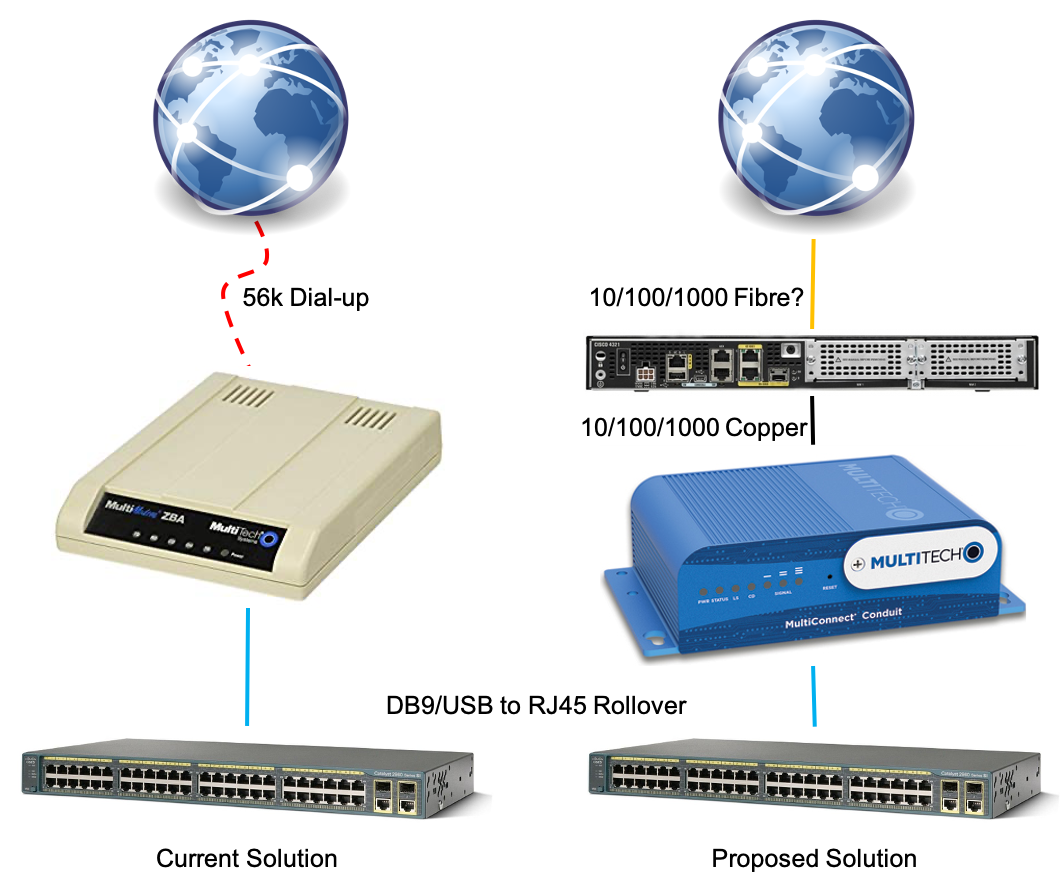
\includegraphics[scale=0.7]{img/3-design/physical.png}
    \captionof{figure}{Physical solution design}
    \label{fig:3-physical}
\end{center}